\chapter{Methodology}

As there are no publically available datasets with images of pain assessment in a fetus, our work was developed in conjunction with the group of studies of Fetal Pain Assessment from the University of São Paulo (USP), which studies pain assessment in fetuses and was responsible for collecting the videos.

Videos were recorded in three groups. The first one was a baseline with fetuses in resting conditions. The second one was of fetuses that had to go through an intra-uterine surgery, and thus needed fetal anesthesia, in this case, the exact moment of the puncture was recorded. This recording captured the reaction of the fetus and its manifestations of pain. These videos had two parts in it, first a baseline period defined as the least 30 seconds before the anesthesia puncture and second the 45 seconds immediately after the puncture. Lastly, the third group of videos was recorded while the fetus was exposed to the sound of a horn, this was meant to cause distress but no harm, thus it serves as a control group different from pain which we expected our method would be able to differentiate. This process collected a total of 15 videos, being five from each group.

% Videos were recorded from the 4D Ultrasound machine of the model Voluson E8 by GE. 

For the images collected during fetal anesthesia, a second ultrasound machine was placed in the clinical room, as the main one was used for the medical procedure of the anesthetic puncture and the second one was used to target the fetus's face to monitor its expressions. These images with a fetus in pain conditions were evaluated by 3 professionals with the NFCS scale, and these evaluations were further used to quantify the amount of pain.

\section{Image Sampling}

It is common to have a small number of data to work with as this is a very hard data to collect. Only a small percentage of pregnancies require intra-uterus intervention prior to birth, and thus fetal anesthesia is a relatively rare procedure. Because of that, it is common for studies in the filed to also have a small N, like these ones cite{}.

To deal with the limited amount of data, we've decided to bring the data to another dimension, we reduced the space from videos to images. In other to do this, we decided to sample the videos at the hate of every 2 seconds. With these processes, we created a total of 268 images.

But as the images were recorded from ultrasound machines, they depend on the calibration by the doctors to capture the exact section of the 3-dimensional space where the fetus face is. Because of this, it is common for this type of image to have a lot of noise, and thus some of the sampled images did not contain a clear face of the fetus. This was a problem, as we had a significant number of images, and manual selection would not only be hard but also non-deterministic.

To overcome this issue, we decided to use a neural network capable of detecting facial landmarks, like the nose, the mouth, and the eyes. The network we used was the Multi-task Cascaded Convolutional Networks (MTCNN) developed by \cite{ZhangZL016} which was created to identify faces in images. It worked surprisingly well in our domain, even though the images had quite different characteristics.

With this process, we were able to filter out our dataset of images from 268 to 145 and we're sure the images contained a clear face. The network also returned a confidence number of which it found the face in the image, and we've used only confidences of over 95\%, which on manual inspection was very reliable, with just 6 errors that were removed manually.

With the position of the facial landmarks, another process was to crop the images around the face of the fetus. This cropping is done just by adding padding to the places where the image was. This process is achivable after we have the positions of the landmarks returned through the MTCNN. This also makes face alignment possible. This way, we avoid the blurred surroundings around the fetus which contains non-distinguishable parts. 

At this point, manual inspection was needed in other to separate the images back into the three groups. With the resting images, it was easy as all the frames were from resting positions. But with the ones from anesthesia and from the horn we had to split the data between before the stimulus and after it. This was not a though process as we knew exactly when the stimuli were applied and a clear difference in the facial expression could be noted. After this step, we ended up with 117 images which had a clear face on it. An example of cropping can be seen on Figure \ref{fig:cropping}.

\begin{figure}[h!tp]
    \centering
    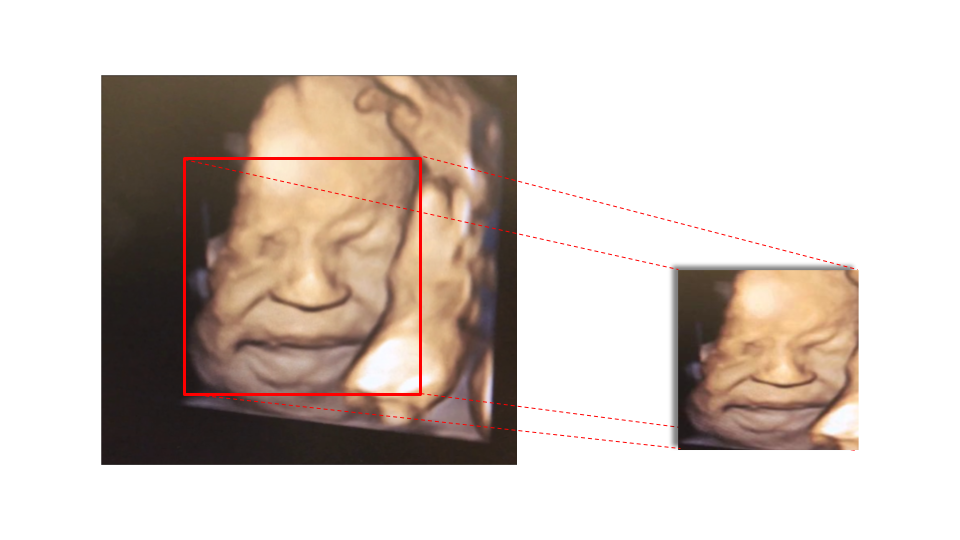
\includegraphics[width=.9\textwidth]{imgs/chap3_cropping.png}
    \caption{Image cropping with MTCNN}
    \label{fig:cropping}
\end{figure}

\section{Data Augmentation}

Even though we had increased the size of the dataset by turning the videos into images, it was still considered a small dataset for deep learning models. To further augment our chances of succeeding, we have applied the use of data augmentation techniques to increase the variability of our data. The effectiveness of such a technique has been demonstrated by \cite{abs-1712-04621} and is widely used in the field.

There is a range of possibilities for using data augmentation, the ones we've chosen are:

* Horizontal flip, which consists of mirroring the image horizontally. 
* Rotation, which consists in applying small rotations to the image.
* Zoom, which consists of zooming in the image.
* Lightning, which consists of changing the brightness and the contrast of the image.
* Warping, which consists of adding distortions to the image. 

All of these methods have a probability of being applied and can be used in combination with each other. Thus for each image, given the probability, a combination of these techniques would be applied. Some examples of these different combinantions of data augmentation with the same image are shown on Figure \ref{fig:data_augmentation}.

\begin{figure}[h!tp]
    \centering
    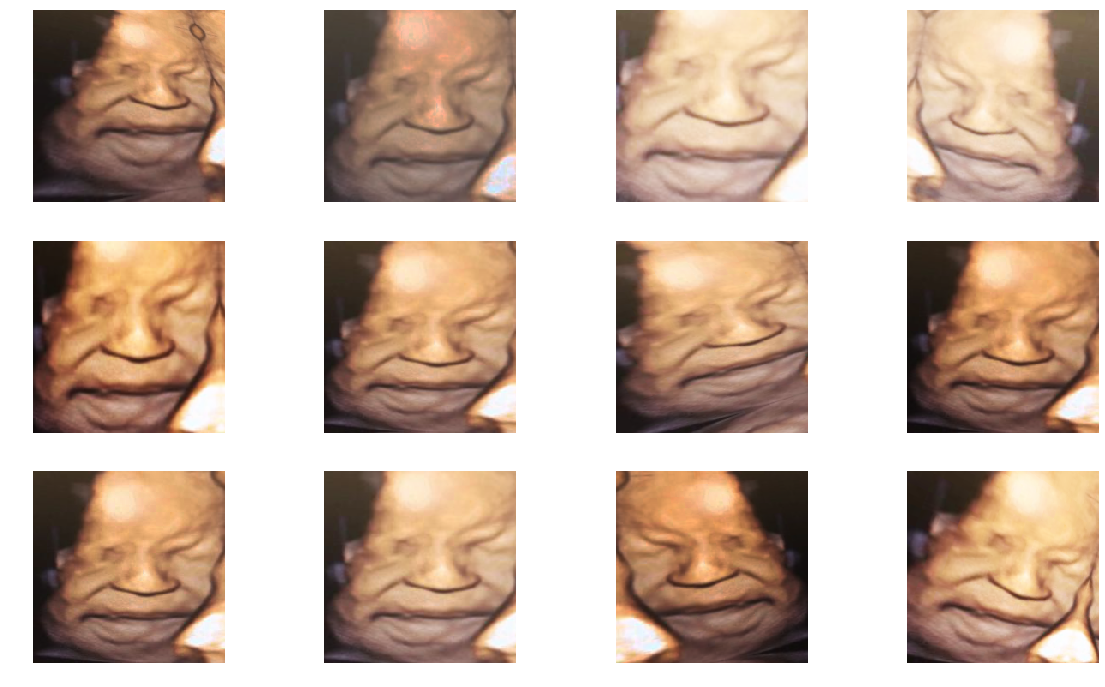
\includegraphics[width=.9\textwidth]{imgs/chap3_data_augmentation.png}
    \caption{The same image with different data augmentation applied}
    \label{fig:data_augmentation}
\end{figure}

To further experiment with this process, we have compared 3 sets of intensity in the changes. A smooth, which does more subtle changes, a medium one, which intensifies a little bit and a more aggressive one, which heavily transforms the images.  

\subsection{Network Architecture and Transfer Learning}

The network used was VGG with a pre-trained model on VGG Face, developed by \cite{ParkhiVZ15}.



